\chapter{The Seifert-Van Kampen Theorem}
Here is the statement of Seifert-Van Kampen Theorem:
\begin{theorem} Let \(K = {K}_{1} \cup  {K}_{2}\) be the union of two path-connected open sets, where \({K}_{1} \cap  {K}_{2}\) is also path-connected. Take \(b \in  {K}_{1} \cap  {K}_{2}\), and suppose the group presentations for \({\pi }_{1}\left( {{K}_{1},b}\right),{\pi }_{1}\left( {{K}_{2},b}\right)\) are
\[
{\pi }_{1}\left( {{K}_{1},b}\right)  \cong  \left\langle  {{X}_{1} \mid  {R}_{1}}\right\rangle ,\;{\pi }_{1}\left( {{K}_{2},b}\right)  \cong  \left\langle  {{X}_{2} \mid  {R}_{2}}\right\rangle .
\]
Let the inclusions be
\[
{i}_{1} : {K}_{1} \cap  {K}_{2} \hookrightarrow  {K}_{1},\;{i}_{2} : {K}_{1} \cap  {K}_{2} \hookrightarrow  {K}_{2},
\]
then a presentation of \({\pi }_{1}\left( {K,b}\right)\) is given by:
\[
{\pi }_{1}\left( {K,b}\right)  \cong  \left\langle  {{X}_{1} \cup  {X}_{2} \mid  {R}_{1} \cup  {R}_{2} \cup  \left\{  {{\left( {i}_{1}\right) }_{ * }\left( g\right)  = {\left( {i}_{2}\right) }_{ * }\left( g\right)  : \forall g \in  {\pi }_{1}\left( {{K}_{1} \cap  {K}_{2},b}\right) }\right\}  }\right\rangle .
\]
(Here \({\left( {i}_{1}\right) }_{ * } : {\pi }_{1}\left( {{K}_{1} \cap  {K}_{2},b}\right)  \hookrightarrow  {\pi }_{1}\left( {{K}_{1},b}\right)\) and \({\left( {i}_{2}\right) }_{ * } : {\pi }_{1}\left( {{K}_{1} \cap  {K}_{2},b}\right)  \hookrightarrow  {\pi }_{1}\left( {{K}_{2},b}\right)\).)
\end{theorem}

\begin{example} Let \(K = {S}^{1} \vee  {S}^{1}\) given by
\begin{center}
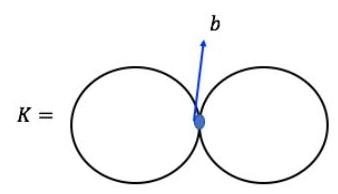
\includegraphics[width=0.2\textwidth]{images/Ch9_S1vS1.jpg}
\end{center}

Let \(b\) be the intersection between two circles, and construct \({K}_{1},{K}_{2}\) as shown below: 

\begin{center}
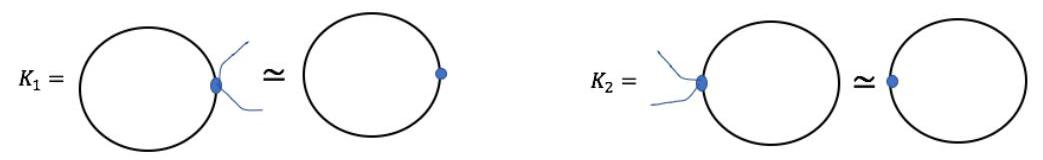
\includegraphics[width=0.8\textwidth]{images/Ch9_K1K2_1.jpg}
\end{center}

We can see that \({K}_{1} \cap  {K}_{2}\) is contractible:
\begin{center}
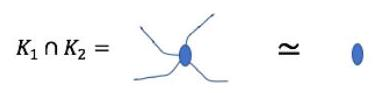
\includegraphics[width=0.5\textwidth]{images/Ch9_K1capK2_1.jpg}
\end{center}
As we proved before, \({\pi }_{1}\left( {S}^{1}\right)  \cong  \mathbb{Z}\), which follows that
\[
{\pi }_{1}\left( {{K}_{1},b}\right)  \cong  \langle \alpha \rangle,\;{\pi }_{1}\left( {{K}_{2},b}\right)  \cong  \langle \beta \rangle
\]
Also, \({\pi }_{1}\left( {{K}_{1} \cap  {K}_{2},b}\right)  \cong  {\pi }_{1}\left( {\{ b\},b}\right)  \cong  \{ e\} \text{. }
\)

Also, it is easy to compute \({\left( {i}_{1}\right) }_{ * }\) and \({\left( {i}_{2}\right) }_{ * }\) : For instance, \({\left( {i}_{2}\right) }_{ * } : \;{\pi }_{1}\left( {{K}_{1} \cap  {K}_{2}}\right)  \rightarrow  {\pi }_{1}\left( {K}_{2}\right)\)
is given by $e \mapsto  e$. 
Therefore, by Seifert-Van Kampen Theorem,
\[
{\pi }_{1}\left( {K,b}\right)  \cong  \langle \alpha,\beta  \mid  e = e\rangle  \cong  \langle \alpha,\beta \rangle
\]

More generally, by induction

\[
{\pi }_{1}\left( {{ \vee  }^{n}{S}^{1},b}\right)  \cong  \left\langle  {{a}_{1},\ldots,{a}_{n}}\right\rangle
\]

For instance, the figure illustration for \({ \vee  }^{4}{S}^{1}\) and the basepoint \(b\) is given below:
\begin{center}
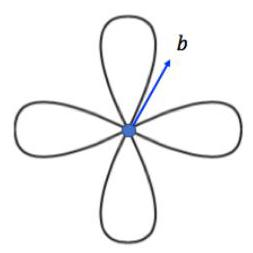
\includegraphics[width=0.35\textwidth]{images/Ch9_4_petals.jpg}
\end{center}
\end{example}

\begin{example}
Consider\({S}^{2} = {K}_{1} \cup  {K}_{2}\), which is shown below:
\begin{center}
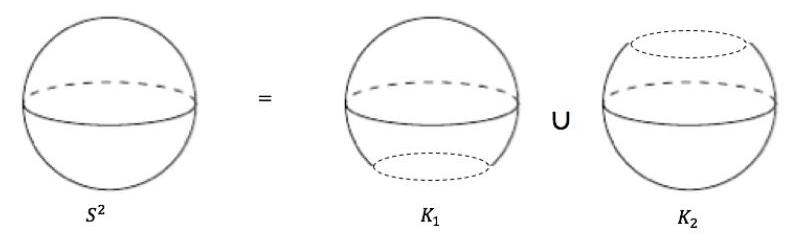
\includegraphics[width=0.8\textwidth]{images/Ch9_S2_K1K2.jpg}
\end{center}
Therefore, we see that \({K}_{1} \cap  {K}_{2} \simeq  {S}^{1}\) :
\begin{center}
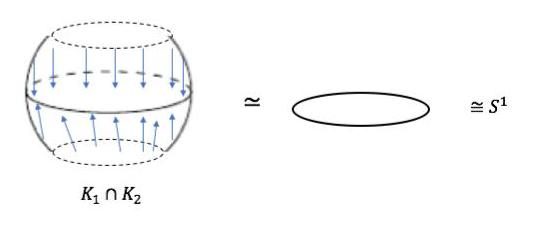
\includegraphics[width=0.6\textwidth]{images/Ch9_S2_K1capK2_S1.jpg}
\end{center}
while \({K}_{1}\) and \({K}_{2}\) are contractible. Therefore
\[
{\pi }_{1}\left( {K}_{1}\right)  \cong  \langle \beta  \mid  \beta \rangle,\;{\pi }_{1}\left( {K}_{2}\right)  \cong  \langle \gamma  \mid  \gamma \rangle
\]
and 
\({\pi }_{1}\left( {{K}_{1} \cap  {K}_{2}}\right)  \cong  {\pi }_{1}\left( {S}^{1}\right)  \cong  \langle \alpha \rangle\).

Now we compute \({\left( {i}_{1}\right) }_{ * }\) and \({\left( {i}_{2}\right) }_{ * }\): 
For any loop \(\gamma\) in $K_1 \cap K_2$ based at \(b\), Since \({K}_{1}\) is contractible, we imply \(\gamma\) in \({K}_{1}\) is homotopic to \({c}_{b}\), i.e.,
\[
{\left( {i}_{1}\right) }_{ * }\left( \left\lbrack  \gamma \right\rbrack  \right)  = \left\lbrack  {{i}_{1}\left( \gamma \right) }\right\rbrack   = e,\forall \gamma  \in  {\pi }_{1}\left( {{K}_{1} \cap  {K}_{2}}\right).
\]
Similarly, \({\left( {i}_{2}\right) }_{ * }\left( \left\lbrack  \gamma \right\rbrack  \right)  = e\).

Therefore, by Seifert-Van Kampen Theorem, we conclude that
\[
{\pi }_{1}\left( {S}^{2}\right)  \cong  \langle \beta,\gamma  \mid  \beta,\gamma,e = e\rangle  \cong  \{ e\}
\]
\end{example}

Homework: Use the same trick to check that \({\pi }_{1}\left( {S}^{n}\right)  = \{ e\}\) for all \(n \geq  2\) (Hint: for \({S}^{3}\), construct
\[
{K}_{1} = \left\{  {\left( {{x}_{1},\ldots,{x}_{4}}\right)  \in  {S}^{3} \mid  {x}_{4} >  - 1/2}\right\}
\]
and
\[
{K}_{1} = \left\{  {\left( {{x}_{1},\ldots,{x}_{4}}\right)  \in  {S}^{3} \mid  {x}_{4} < 1/2}\right\})
\]

\begin{example}
Consider \(K \cong  {\mathbb{T}}^{2}\), and \(K = {K}_{1} \cup  {K}_{2}\) given by:
\begin{center}
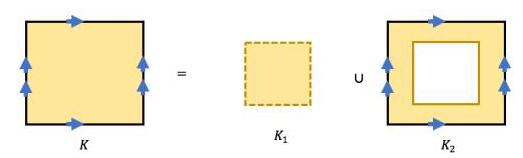
\includegraphics[width=0.6\textwidth]{images/Ch9_T_K1K2.jpg}
\end{center}
Therefore, we can see that \({K}_{1}\) is contractible, and \({K}_{2}\) is homotopy equivalent
to \({S}^{1} \vee  {S}^{1}\) :
\begin{center}
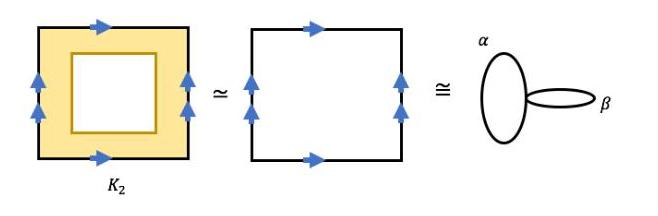
\includegraphics[width=0.6\textwidth]{images/Ch9_T_K1capK2.jpg}
\end{center}
and \({K}_{1} \cap  {K}_{2}\) is homotopic equivalent to the circle:
\begin{center}
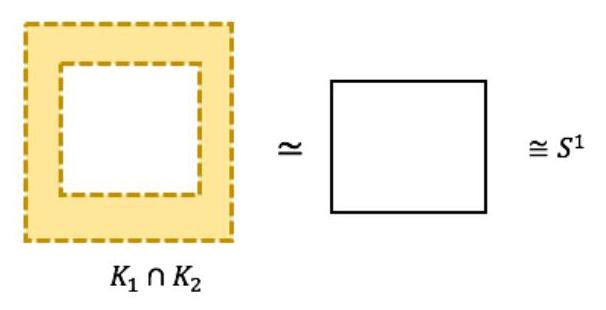
\includegraphics[width=0.6\textwidth]{images/Ch9_T_K1capK2_2.jpg}
\end{center}
It follows that
\[
{\pi }_{1}\left( {K}_{1}\right)  \cong  \{ e\},\;{\pi }_{1}\left( {K}_{2}\right)  \cong  \langle \alpha,\beta \rangle,\ {\pi }_{1}\left( {{K}_{1} \cap  {K}_{2}}\right)  \cong  \langle \gamma \rangle.\]
Then we compute \({\left( {i}_{1}\right) }_{ * }\) and \({\left( {i}_{2}\right) }_{ * }\). Firstly, \({\left( {i}_{1}\right) }_{ * }\) is trivial as in the previous example:
\[
{\left( {i}_{1}\right) }_{ * } : \;{\pi }_{1}\left( {{K}_{1} \cap  {K}_{2}}\right)  \rightarrow  {\pi }_{1}\left( {K}_{1}\right)
\ \text{ with }\left\lbrack  \alpha \right\rbrack   \mapsto  e
\]
As for \({\left( {i}_{2}\right) }_{ * }\), let \(\gamma\) be any loop in $K_1 \cap K_2$. We draw the graph for \({i}_{2}\left( \gamma \right)\) :
\begin{center}
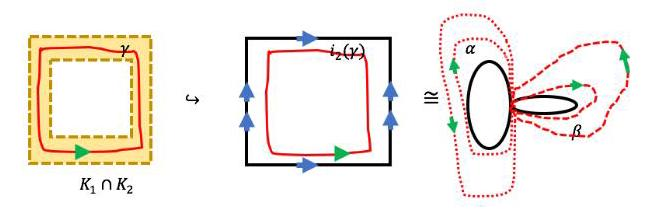
\includegraphics[width=0.8\textwidth]{images/Ch9_K12_into_K2.jpg}
\end{center}
Therefore,
\[
{\left( {i}_{2}\right) }_{ * }\left\lbrack  \gamma \right\rbrack   = \left\lbrack  {{i}_{2}\left( \gamma \right) }\right\rbrack   = \left\lbrack  {{\alpha \beta }{\alpha }^{-1}{\beta }^{-1}}\right\rbrack
\]
And by Seifert-Van Kampen Theorem, we conclude that
\[
{\pi }_{1}\left( K\right)  \cong  \left\langle  {\alpha,\beta  \mid  \beta,{\alpha \beta }{\alpha }^{-1}{\beta }^{-1} = e}\right\rangle   \cong  \langle \alpha,\beta  \mid ,{\alpha \beta } = {\beta \alpha }\rangle  \cong  \mathbb{Z} \times  \mathbb{Z}
\]
\end{example}

Exercise: The Klein bottle \(K\) shown in graph below satisfies \({\pi }_{1}\left( K\right)  = \left\langle  {a,b \mid  {ab}{a}^{-1}b}\right\rangle\).
\begin{center}
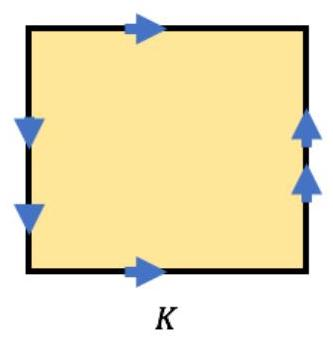
\includegraphics[width=0.35\textwidth]{images/Ch9_Klein.jpg}
\end{center}

\begin{example}
Consider the space \(K = \mathbb{R}{P}^{2}\) with \(K = {K}_{2} \cup  {K}_{2}\) given by:
\begin{center}
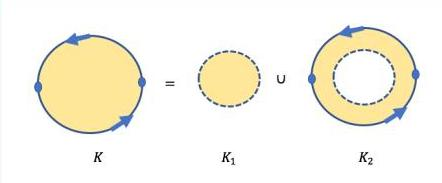
\includegraphics[width=0.7\textwidth]{images/Ch9_RP2_K1K2.jpg}
\end{center}
It is clear that \({K}_{1}\) is contractible. And in Homework 3, we can see that \({K}_{2} \simeq  {S}^{1}\). Moreover, \({K}_{1} \cap  {K}_{2} \simeq  {S}^{1}\) as before. Therefore, 
\[{\pi }_{1}\left( {K}_{1}\right)  = \{ e\},\ {\pi }_{1}\left( {K}_{2}\right)  = \langle \alpha \rangle,\ {\pi }_{1}\left( {{K}_{1} \cap  {K}_{2}}\right)  = \langle \gamma \rangle.\]
It’s easy to see that \({\left( {i}_{1}\right) }_{ * }\left( \left\lbrack  \gamma \right\rbrack  \right)  = e\) for any loop \(\gamma\). As for \({\left( {i}_{2}\right) }_{ * }\left( \left\lbrack  \gamma \right\rbrack  \right)\):
\begin{center}
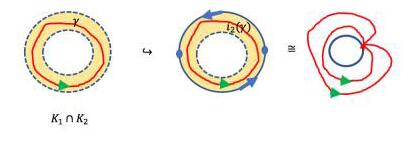
\includegraphics[width=0.7\textwidth]{images/Ch9_RP2_i2star.jpg}
\end{center}
Therefore, \({\left( {i}_{2}\right) }_{ * }\left( \left\lbrack  \gamma \right\rbrack  \right)  = \left\lbrack  {{i}_{2}\left( \gamma \right) }\right\rbrack   = \left\lbrack  {\alpha }^{2}\right\rbrack\).

By Seifert-Van Kampen Theorem, we conclude that
\[
{\pi }_{1}\left( K\right)  \cong  \left\langle  {\alpha  \mid  {\alpha }^{2} = e}\right\rangle   \cong  \mathbb{Z}/2\mathbb{Z}
\]
\end{example}

\begin{example}
Let \(K = {\mathbb{R}}^{2} \smallsetminus  \{ 2\) points \(\alpha,\beta \}\). As we have shown in Homework 3, \(K \simeq  {S}^{1} \vee  {S}^{1}\), which implies
\[
{\pi }_{1}\left( K\right)  \cong  {\pi }_{1}\left( {{S}^{1} \land  {S}^{1}}\right)  \cong  \langle \alpha,\beta \rangle.
\]

We can compute the fundamental group for \(K\) using Seifert-Van Kampen Theorem directly: Construct \(K = {K}_{1} \cup  {K}_{2}\) as follows:
\begin{center}
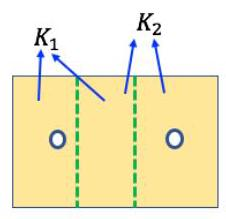
\includegraphics[width=0.3\textwidth]{images/Ch9_lasteg_K1K2.jpg}
\end{center}
It is clear that \({K}_{1} \cong  {\mathbb{R}}^{2} \smallsetminus  \{\) one point \(\}  \simeq  {S}^{1}\) and similarly \({K}_{2} \simeq  {S}^{1}\). Moreover, \({K}_{1} \cap  {K}_{2}\) is contractible. Therefore,
\[
{\pi }_{1}\left( {K}_{1}\right)  \cong  \langle \alpha \rangle,\;{\pi }_{1}\left( {K}_{2}\right)  \cong  \langle \beta \rangle,\;{\pi }_{1}\left( {{K}_{1} \cap  {K}_{2}}\right)  \cong  \{ e\}
\]
Also, \({\left( {i}_{1}\right) }_{ * }\) and \({\left( {i}_{2}\right) }_{ * }\) is trivial, since \({\pi }_{1}\left( {{K}_{1} \cap  {K}_{2}}\right)  \cong  \{ e\}\).

By Seifert-Van Kampen Theorem, we conclude that
\[
{\pi }_{1}\left( K\right)  \cong  \langle \alpha,\beta  \mid  e = e\rangle  \cong  \langle \alpha,\beta \rangle
\]
\end{example}